\newcommand{\lub}{\ensuremath{\sqcup}\xspace}
\newcommand{\Lub}{\ensuremath{\bigsqcup}\xspace}
\newcommand{\state}{\ensuremath{\mathit{s}}\xspace}
\newcommand{\STG}{\ensuremath{\mathrm{STG}}\xspace}
\newcommand{\States}{\ensuremath{\mathit{States}}\xspace}
\newcommand{\prop}[1]{\ensuremath{p_{\state,#1}}\xspace} 
\newcommand{\propp}[1]{\ensuremath{p_{\state',#1}}\xspace} 
\newcommand{\G}{\ensuremath{\mathrm{G}}\xspace}
\newcommand{\F}{\ensuremath{\mathrm{F}}\xspace}
\newcommand{\X}{\ensuremath{\mathrm{X}}\xspace}
\newcommand{\R}{\ensuremath{\mathrm{R}}\xspace}
\newcommand{\U}{\ensuremath{\mathrm{U}}\xspace}
\newcommand{\WU}{\ensuremath{\mathrm{WU}\xspace}}
\newcommand{\comb}{\ensuremath{\mathit{joined\_succs}}\xspace}


\begin{frame}{Linear Time Logic Formul\ae\ Verification}

  \begin{block}{Data-flow based approach}
    \begin{itemize}
    \item[-] lossy approximation (upper bound in Boolean lattice)
    \item[+] Very fast
    \end{itemize}
  \end{block}

  \begin{block}{Algorithm 1/2}
    \footnotesize
    \begin{algorithm}[H]
      \SetLine
      \KwIn{State Transition Graph}
      \KwOut{Formulae true, false, or unknown.}

      $G_1$=collapse(STG) \Comment{remove all non-I/O nodes and all exit (=assert) nodes}\\
      eval(LTL, $G_1$) \Comment{Evaluate all LTL sub-expressions bottom-up}
    \end{algorithm}
  \end{block}
\end{frame}

\begin{frame}{Linear Time Logic Formul\ae\ Verification 2}
  \begin{block}{LTL evaluation function}

    \scriptsize
    \newcommand{\ALLS}{\quad\forall\state\in\States\colon}
  \begin{algorithm}[H]
    \SetLine
    \KwIn{LTL expression, State Transition Graph}
    \KwOut{$\state\in\States\rightarrow$ BoolLattice}
    \textbf{function} eval(e, g)\\
    \Begin{
        \Switch{e}{
          \lCase{$a\ \&\ b$}{$\!\colon\quad eval(a, G); eval(b, G);\ALLS s_e = s_a \cap s_b$}\\
          \lCase{$a\ |\  b\:$}{$\colon\quad eval(a, G); eval(b, G);\ALLS s_e = s_a \cup s_b$}\\
          \lCase{$!a\quad\;\,$}{$\colon\quad eval(a, G);\ALLS s_e = \neg s_a$}\\
          \lCase{$\X a\quad$}{$\colon\quad eval(a, G);\ALLS s_e=\Lub_{\state\prime\in succ(\state)}s'_a$}\\
          \lCase{$\G a\quad$}{$\colon\quad$fix($\bot, \lub, \lambda s,\comb\colon s_a\cap\comb$)}\\
          \lCase{$\F a\quad\:$}{$\colon\quad$fix($\bot, \lub, \lambda s,\comb\colon s_a\cup\comb)$}\\
          \lCase{a \R b}{$\colon\quad$fix($\bot, \lub, \lambda s,\comb\colon s_b\cap(s_a\cup\comb))$}\\
          \lCase{a \U b}{$\colon\quad$fix($\bot, \lub, \lambda s,\comb\colon s_b\cup(s_a\cap\comb))$}\\
          \lCase{a \WU\ b}{: eval(G a $|$ (a \U b), g)}\\
        }
      }
      
      \caption{eval}
    \end{algorithm}

    \medskip

    worklist/fixpoint:  fix(\emph{init}, \emph{join}, \emph{transfer})\\
    \comb: $\Lub_{\state\prime\in succ(\state)}s'_e$ (joined result of successors of s)\\
  \end{block}
\end{frame}
\newcommand{\ffalse}{\ensuremath{\mathit{false}}}
\newcommand{\ttrue}{\ensuremath{\mathit{true}}}




\begin{frame}{Linear Time Logic Formul\ae\ Verification}

  \begin{block}{Unified approach}
    \begin{itemize}
    \item[+] precise (explores all states, no merging)
    \item[-] Slower than fixpoint, more memory
    \end{itemize}
  \end{block}
\end{frame}

\begin{frame}{Order of evaluation}{}
{\bf Input:} $ \neg o(U)\ WU\ (o(Z) \wedge \neg o(U)) $\\
\begin{block}{de-sugar}
de-sugar $WU$: $ x\ WU\ y \rightarrow G x \vee (x\ U\ y)$\\
\end{block}
\begin{block}{resulting LTL expression DAG}
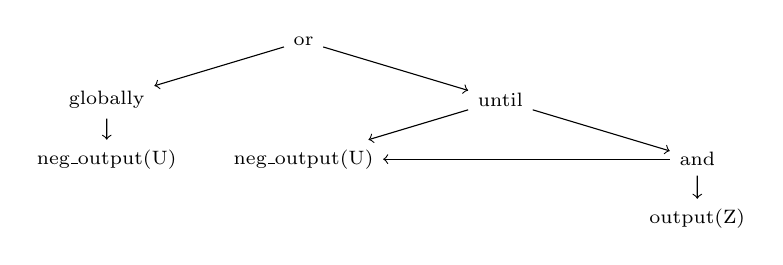
\begin{tikzpicture}[->,n/.style={font=\scriptsize},level
    distance=.75cm,sibling distance=5cm] 
\node[n] {or}
    child{ node[n] {globally} 
      child{ node[n] {neg\_output(U)} }
    }
    child{ node[n] {until}
      child{ node[n] (nu) {neg\_output(U)} }
      child{ node[n] (and) {and}
        child{ node[n] {output(Z)} }
      }
    }
;
\draw (and) -> (nu);
\end{tikzpicture}
\end{block}

\begin{block}{LTL value-stack operations (in postfix notation)}
\texttt{\footnotesize neg\_output(U) G neg\_output(U) dup output(Z) and until or}
\end{block}
\end{frame}



\begin{frame}{Linear Time Logic Formul\ae\ Verification}
  \begin{block}{Algorithm}
    \scriptsize
    \begin{algorithm}[H]
      \SetLine
      \KwIn{State Transition Graph (collapsed)}
      \KwOut{Formulae true, false, or unknown.}
      \lForEach{S $\in$ STG}{ 
        \{ val$_S$ = $\bot$; W = W $\cup$ S \} } \;
      \While{W $\neq$ $\emptyset$}{
         W = W $\setminus$ succ; \Comment{take succ from worklist}\\
         %remove\_if\_orphan(succ)\;
         \ForEach{S $\in$ pred(succ)}{
            val' := transfer(S, val$_\mathit{succ}$); 
            \Comment{compute the transfer function for S}\\
            \lIf{val$_S$ == val'}{
               continue; \Comment{Reached fixpoint}\;
            }
            \Else{
               S' := add\_state\_if\_new(S, val'), val$_{S'}$ = val' \;
               add\_edge(S', succ); \Comment{self-cycles not shown}\\
               remove\_edge(S, succ); \Comment{patch up the new state}\\
               
               \lForEach{pred $\in$ pred(S)}{
                  add\_edge(pred, S')\;
               }
               \lForEach{succ $\in$ succ(S)}{
                  W := W $\cup$ succ; \Comment{add other succs of old S}\\
               }
               W := W $\cup$ S\;
            }
         }
      }
      \ForEach{S $\in$ STG}{
        \lFor{i := 0 .. nargs}{
          valstack$_S$.pop(); \Comment{consume args on valstack}\\
          valstack$_S$.push(val$_S$)\;
        }
      }
    \end{algorithm}
  \end{block}
\end{frame}

\newcommand{\minibox}[2]{\begin{minipage}{#1}#2\end{minipage}}
\begin{frame}{Unified algorithm visualized}{}
\begin{block}{Example: computing $F\ x$, $\mathit{worklist} = \{\dots,b\}$}
  \begin{tikzpicture}[->,
      n/.style={draw,font=\scriptsize},
      new/.style={green,thick},
      cut/.style={dashed,red,thick},
      level distance=1.5cm,sibling distance=4cm] 
  \node[n] (a) {$a$: [ 0 ] $\bot$}
        child[draw=bg] { node[] (ghost) {\large\usebeamercolor[bg]{[$'$]}} }
        child{ node[n]  (s) {$S$:  [ 0 ] 0 } 
          child{ node[n,red] (b) {$b$: [ 1 ] 1 } }
          child{ node[n] (c) {$c$: [ 0 ] $\bot$} }
        }
  ;
  \node[right of=a, node distance=3.5cm]{\tiny\bf Legend: };
  \node[right of=a, node distance=6cm,draw]{\tiny Node: [ value-stack ] next-top-of-stack };
  \node[below of=c, node distance=1em]{\tiny not yet visited};
  \node[below of=b, node distance=1em]{\tiny top of worklist};
  \pause
  \node[n,left of=ghost, node distance=0cm,new] (s1) {$S'$: [ 0 ] 1 };
  \node[below of=s1, node distance=1em]{\tiny recomputed S'};
  \pause
  \draw[new] (a) -> (s1);
  \draw[new] (s1) -> (b);
  \draw[new] (s1) -> (c);
  \pause
  \draw[cut] (s) -> (b);
  \node[below left of=s, node distance=1.5cm,red]{\tiny$\quad$ cut off};
  \end{tikzpicture}
\end{block}
\footnotesize
\begin{enumerate}
\item<1->{Take $b$ from worklist\\}
\item<2->{ 
  Create $S' \neq S$
  \scriptsize
  ($\mathit{transfer\_F}(\mathit{succ}, \mathit{val}) = \mathit{succ} \vee \mathit{val}$,
  $\mathit{transfer\_F}(1, 0) = 1$)\\
}
\item<3->{patch up S'\\}
\item<4->{cut off the part of $S$ that is now represented by $S'$\\}
\item<5->{$\mathit{worklist} = \mathit{worklist} \cup \{S', c\}$}
\end{enumerate}
\end{frame}



\begin{frame}{Backup slide: Operators}
  \begin{block}{Boolean lattice the LTL formul\ae\ are reduced to}
    \begin{columns}
      \begin{column}{4cm}
   \begin{tikzpicture}[scale=.9]
    \small
    \node (top) {$\top$} 
    child {node (-1)    {\ffalse}}
    child {node (0)     {}
      edge from parent[draw=none]
      child {node (bot) {$\bot$} 
      edge from parent[draw=none]
      }
    }
    child {node (1)    {\ttrue}} 
    ; 
    \draw (-1)    -- (bot);
    \draw (1)     -- (bot);
  \end{tikzpicture} 
\end{column}
\begin{column}{6cm}
  \scriptsize
  \begin{tabular}{r|llll}
    \lub   & $\bot$ & \ffalse & \ttrue & $\top$ \\ \hline
    $\bot$ & $\bot$ & \ffalse & \ttrue & $\top$ \\
    \ffalse& \ffalse& $\top$  & $\top$ & $\top$ \\
    \ttrue & \ttrue & $\top$  & $\top$ & $\top$ \\
    $\top$ & $\top$ & $\top$  & $\top$ & $\top$ \\
  \end{tabular}\\
  \medskip
  \begin{tabular}{r|llll}
    $\cap$ & $\bot$ & \ffalse & \ttrue & $\top$ \\ \hline
    $\bot$ & $\bot$ & \ffalse & \ttrue & $\top$ \\
    \ffalse& \ffalse& \ffalse & \ffalse& \ffalse \\
    \ttrue & \ttrue & \ffalse & \ttrue & $\top$ \\
    $\top$ & $\top$ & \ffalse & $\top$ & $\top$ \\
  \end{tabular}\\
  \medskip
  \begin{tabular}{r|llll}
    $\cup$ & $\bot$ & \ffalse & \ttrue & $\top$ \\ \hline
    $\bot$ & $\bot$ & \ffalse & \ttrue & $\top$ \\
    \ffalse& \ffalse& \ffalse & \ttrue & $\top$ \\
    \ttrue & \ttrue & \ttrue  & \ttrue & \ttrue \\
    $\top$ & $\top$ & $\top$  & \ttrue & $\top$ \\
  \end{tabular}

\end{column}
    \end{columns}
  \end{block}
\end{frame}

\begin{frame}{Finding Counterexamples with QuickCheck 1/2}
  \begin{block}{Motivation}
    \begin{itemize}
    \item Needed a way to verify verification results
    \item Idea: use the executable to find concrete counterexamples
    \item Intended to verify correctness of \emph{false} results
    \item But turned out to be quite effective!
    \end{itemize}
  \end{block}

  \begin{block}{Idea}
    \begin{itemize}
    \item Use QuickCheck to generate random inputs
    \item Execute program to generate a specific output sequence
    \item verify LTL on I/O sequence $\ffalse \rightarrow$ counterexample!
    \end{itemize}
  \end{block}
\end{frame}

\begin{frame}[fragile]{Finding Counterexamples with QuickCheck 2/2}
  \begin{block}{Implementation}
    \begin{itemize}
    \item $\sim$ 200 lines of Haskell
    \item ignores runs that fail (RERS requirement)
    % Problem: we get only a finite I/O sequence from a run
    % how can we ensure that the result is correct?
    \item operates on Bool lattice to deal with finite I/O sequences:\\
      $\neq\top\rightarrow$ later states cannot influence result 
    \end{itemize}
  \end{block}

  \begin{lstlisting}[language=Haskell,basicstyle=\tiny]
holds :: LTL -> [State] -> BoolLattice
holds (In  c) ((StIn  stc):_) = lift (c == stc)
holds (Out c) ((StOut stc):_) = lift (c == stc)
holds (In  c) ((StOut stc):states) = holds (In  c) states
holds (Out c) ((StIn  stc):states) = holds (Out c) states
holds       (X a) (_:states) = holds a states
holds       (F a) states = (holds a states) ||| (holds (X (F a)) states)
holds       (G a) states = (holds a states) &&& (holds (X (G a)) states)
holds     (Not a) states = nnot (holds a states)
holds (a `And` b) states = (holds a states) &&& (holds b states)
holds (a `Or`  b) states = (holds a states) ||| (holds b states)
holds (a `U`   b) states = (holds b states) ||| ((holds a states) &&& (holds (X (a `U` b)) states))
holds (a `R`   b) states = (holds b states) &&& ((holds a states) ||| (holds (X (a `R` b)) states))
holds (a `WU`  b) states = holds ((G a) `Or` (a `U` b)) states
holds _ _ = Top
  \end{lstlisting}

\end{frame}

\begin{frame}{Work-in-progress:}
  \begin{block}{Motivation}
    Currently precision is lost when two paths merge at a state,
    because we join the information using \lub\ (least upper bound).
  \end{block}
  \begin{block}{Idea}
    \begin{itemize}
    \item Create a new (LTL-)State, instead of joining the two paths.
    \item Identical (LTL-)States will be merged, because they (by
      definition) share the same future/state/successors.
    \end{itemize} 
    Hope to have results by the end of the week!
  \end{block}
\end{frame}
